\section{IOS Modes and Navigation}

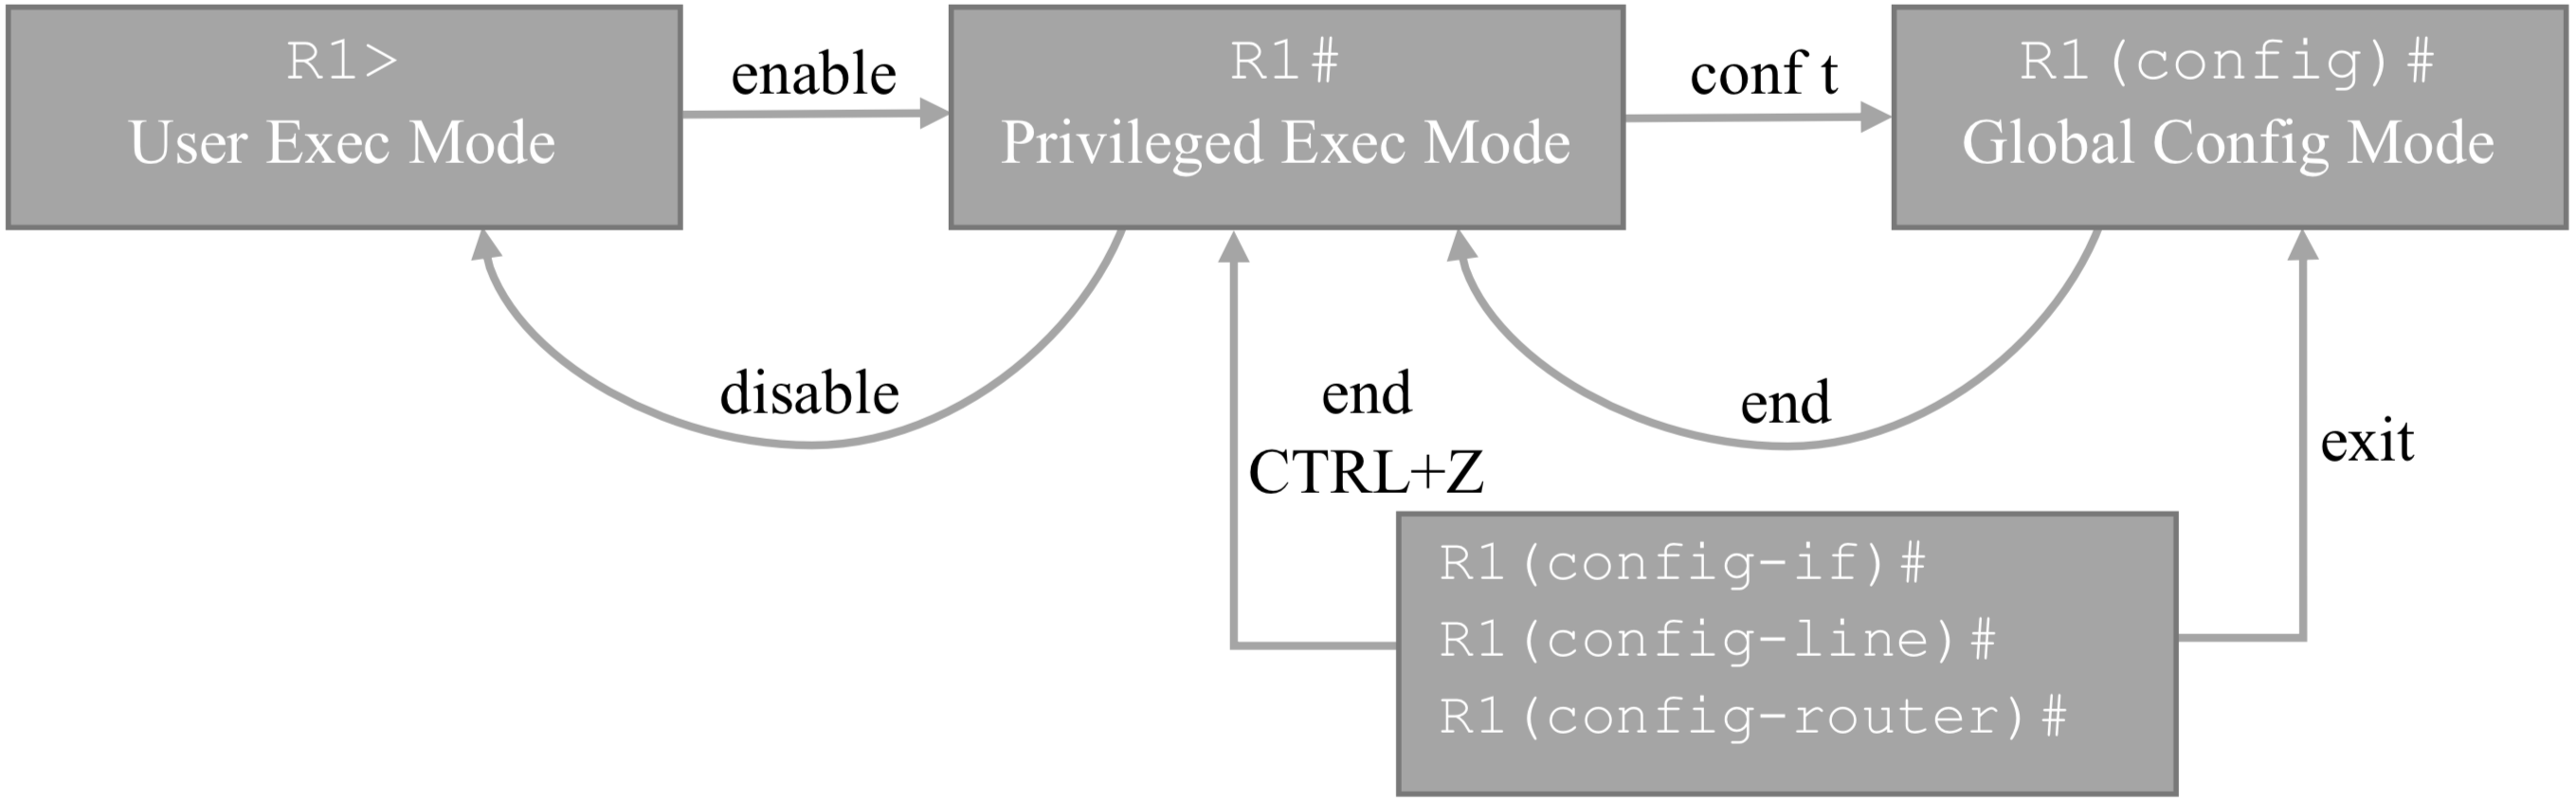
\includegraphics[width=\textwidth]{pics/mode-and-nav}

\noindent
When describing the use of commands, I generally use the conventions shown in \autoref{tab:ioscommandstructure}

\begin{table}[h]
{\tabulinesep=1mm			%Does something with space between rows
\parindent0pt				%No indentation for the table
\begin{tabu}{ | l | X | }
	\hline
	\texttt{Normal/\textbf{Bold}} & Normal/\textbf{Bold} text indicates commands and keywords that you enter literally as shown.\\ \hline
	\texttt{\textit{Italics}} & Italic text indicates arguments for which you supply values. \\ \hline
	\texttt{[x]} & Square brackets indicate an optional element (keyword or argument). \\ \hline
	\texttt{\{x\}} & Braces indiacte a required element (keyword or argument). \\ \hline
	\texttt{[x\{y|z\}]} & Braces and vertical lines within square brackets indicate a required choice within an optional element. \\
	\hline

\end{tabu}}
	\caption{}
	\label{tab:ioscommandstructure}
\end{table}

\section{Basic Setup}
\subsection{Hostname}
\ttfamily
	(config)\# hostname \textit{hostname} \\
	(config)\# hostname no hostname\footnote{Removes the hostname.}
	
\subsection{User Exec Password}
	(config)\# line console 0\textrm{\footnote{0 indicates the first, and properly only console port.}} \\
	(config-line)\# password \textit{password} \\
	(config-line)\# login\footnote{Enables user EXEC access} \\
	(config-line)\# exit
	
\subsection{Privileged Exec Password}
	(config)\# enable secret \textit{secret\_password}\\
	(config)\# exit
	
\subsection{VTY Line Password}
	(config)\# line vty 0 15 \\
	(config-line)\# password \textit{password} \\
	(config-line)\# login\footnote{Enables VTY access}

\subsection{Encrypt Passwords}
(config)\# service password-encryption

\subsection{SVI (Switch Virtual Interface) Configuration}
(config)\# interface vlan \textit{vlan\_id} \\
(config-if)\# ip address \textit{ip\_address} \textit{subnetmask} \\
(config-if)\# no shutdown

\subsection{Default Gateway on a Switch}
(config)\# ip default-gateway \textit{gateway\_address}

\subsection{Description on an interface}
(config-if)\# description \textit{desired\_description}

\subsection{Enable Router to forward IPv6 packets}
(config)\# ipv6 unicast-routing

\subsection{IPv6 link-local}
(config-if)\# ipv6 address \textit{ipv6\_address} link-local

\subsection{Banner Message}
(config)\# banner motd \# hello, this is the message. Choose a \\character that will start and end the message text, in this \\case the hashtag \#

\subsection{Save running config}
\# Copy running-config startup-config
